\documentclass[a4paper,12pt,oneside,onecolum,final,openany]{report} 

%---- Allgemeine Layout Einstellungen ------------------------------------------

% Für Kopf und Fußzeilen, siehe auch KOMA-Skript Doku
\usepackage[komastyle]{scrpage2}
\pagestyle{plain}
\setheadsepline{0.5pt}[\color{black}]
\automark[section]{chapter}


%Einstellungen für Figuren- und Tabellenbeschriftungen
\usepackage[utf8x]{inputenc} 
\usepackage[T1]{fontenc} 
\usepackage[ngerman]{babel} 
\usepackage{amsfonts} 
\usepackage{amsmath} 
\usepackage{tabularx}
\usepackage{float}

%---- Weitere Pakete -----------------------------------------------------------
% Die Pakete sind alle in der TeX Live Distribution enthalten. Wichtige Adressen
% www.ctan.org, www.dante.de

% Sprachunterstützung
\usepackage[ngerman]{babel}

% Benutzung von Umlauten direkt im Text
% entweder "latin1" oder "utf8"
%\usepackage[utf8]{inputenc}

% Pakete mit Mathesymbolen und zur Beseitigung von Schwächen der Mathe-Umgebung
%\usepackage{latexsym,exscale,stmaryrd,amssymb,amsmath}


\usepackage[nointegrals]{wasysym}
\usepackage{eurosym}

% Anderes Literaturverzeichnisformat
%\usepackage[square,sort&compress]{natbib}
\usepackage{hyperref}
% Für Farbe
\usepackage{color}
\usepackage{graphicx}
\usepackage{wrapfig}
\usepackage{subfigure}

% Caption neben Abbildung
\usepackage{sidecap}


% Befehl für "Entspricht"-Zeichen
\newcommand{\corresponds}{\ensuremath{\mathrel{\widehat{=}}}}
% Befehl für Errorfunction
\newcommand{\erf}[1]{\text{ erf}\ensuremath{\left( #1 \right)}}


%Fußnoten zwingend auf diese Seite setzen
\interfootnotelinepenalty=1000

%Für chemische Formeln (von www.dante.de)
%% Anpassung an LaTeX(2e) von Bernd Raichle
\makeatletter
\DeclareRobustCommand{\chemical}[1]{%
  {\(\m@th
   \edef\resetfontdimens{\noexpand\)%
       \fontdimen16\textfont2=\the\fontdimen16\textfont2
       \fontdimen17\textfont2=\the\fontdimen17\textfont2\relax}%
   \fontdimen16\textfont2=2.7pt \fontdimen17\textfont2=2.7pt
   \mathrm{#1}%
   \resetfontdimens}}
\makeatother
\usepackage{textcomp}
\usepackage{upgreek}
%\begin{document}
%$\upmu$
%\end{document}
%Honecker-Kasten mit $$\shadowbox{$xxxx$}$$
\usepackage{fancybox}

%SI-Package
\usepackage{siunitx}

%keine Einrückung, wenn Latex doppelte Leerzeile
\parindent0pt

%Bibliography \bibliography{literatur} und \cite{gerthsen}
%\usepackage{cite}
\usepackage{babelbib}
\selectbiblanguage{ngerman}

\usepackage{siunitx}
%\begin{document}
 % \SI{1.55}{\micro\metre}
\sisetup{math-micro=\text{µ},text-micro=µ}
\usepackage{amsmath}
\usepackage[verbose]{placeins}
\usepackage{setspace}
\usepackage{threeparttable}



\begin{document}

\begin{titlepage}
\centering
\textsc{\Large Physikalisch- Chemisches Grundpraktikum\\[1.5ex] Universität Göttingen}

\vspace*{0.5cm}

\rule{\textwidth}{1pt}\\[0.5cm]
{\huge \bfseries
  Versuch 12: \\[1.5ex]
  Joule-Thomson-Effekt}\\[0.5cm]
\rule{\textwidth}{1pt}

\vspace*{0.5cm}


\begin{Large}
\begin{tabular}{ll}
Durchführende: &  Isaac Maksso, Julia Stachowiak\\
Assistentin: & Katharina Meyer \\
 Versuchsdatum: & 27.10.2016\\
 Datum der ersten Abgabe: & 03.11.2016\\
 Datum der zweiten Abgabe: & 14.11.2016\\
\end{tabular}
\end{Large}

\vspace*{0.5cm}

% Messergebnisse:\\
%\begin{table}[h]
%\centering 
% \begin{tabular}{c|c|c|c|c}
% Temperatur/~°C&$\mu_{\text{N$_{2}$,exp.}}$/~$\frac{\text{K}}{\text{bar}}$&$\mu_{\text{CO$_{2}$,exp.}}$/~$\frac{\text{K}}{\text{bar}}$&$\mu_{\text{N$_{2}$,th.}}$/~$\frac{\text{K}}{\text{bar}}$&$\mu_{\text{CO$_{2}$,th.}}$/~$\frac{\text{K}}{\text{bar}}$\\
% \hline
% 0,1 &1.20±0.04&0.181±0.02&0,0396&0,106\\
% \hline
% 20,7 ($N_2$) bzw. 22,8($CO_2$) &1.01±0.06&0.175±0.02&0,0345&0,0926\\
%\hline 
%50,8 &0.710±0.05&0.120±0.01&0,0272 &0,0771\\
% \end{tabular}
%\end{table}
% Literaturwerte:\\
%\begin{table}[h]
%\centering
%\begin{tabular}{c|c|c}
 % Temperatur/~°C &$\mu_{\text{N$_{2}$,Lit.}}$/~$\frac{\text{K}}{\text{bar}}$&$\mu_{\text{CO$_{2}$,Lit.}}$/~$\frac{\text{K}}{\text{bar}}$\\
%\hline
 %0~°C &$0.26^{1}$ & $1.31^1$\tnote{1}\\
 
%\hline
%20~°C&$0.25^{2}$& $1.12^2$\tnote{2}\\
%\hline
%50~°C&$0.19^{1}$ &$0.91^1$\tnote{1}\\
%\end{tabular}
%\end{table} 

\begin{table}[h]
\centering
\caption{Werte des Joule-Thomson-Koeffizienten für $\text{N}_2$.}
\begin{scriptsize}
\begin{tabular}{c|c|c|c} 
Temperatur/~°C&$ \mu_{\text{N$_{2}$,exp.}}$/~$\frac{\text{K}}{\text{bar}}$&$ \mu_{\text{N$_{2}$,th.}}$/~$\frac{\text{K}}{\text{bar}}$&$ \mu_{\text{N$_{2}$,Lit.}}$/~$\frac{\text{K}}{\text{bar}}$\\
\hline
0,1 & 0,181 $\pm$ 0,02& 0,252 &0,26$^1$\\
\hline
22,7 & 0,175 $\pm$ 0,02& 0,220&0,25$^2$\\
\hline
50,8& 0,120 $\pm$ 0,01& 0,173&0,19$^1$\\
\end{tabular}
\end{scriptsize}
\end{table}
\noindent
\FloatBarrier

\begin{table}[h]
\centering
\caption{Werte des Joule-Thomson-Koeffizienten für $\text{CO}_2$.}
\begin{scriptsize}
\begin{tabular}{c|c|c|c} 
Temperatur/~°C&$ \mu_{\text{CO$_{2}$,exp.}}$/~$\frac{\text{K}}{\text{bar}}$&$ \mu_{\text{CO$_{2}$,th.}}$/~$\frac{\text{K}}{\text{bar}}$&$ \mu_{\text{CO$_{2}$,Lit.}}$/~$\frac{\text{K}}{\text{bar}}$\\
\hline
0,1 & 1,20 $\pm$ 0,04& 1,21&1,31$^1$\\
\hline
22,8 & 1,01 $\pm$ 0,06& 1,05&1,12$^2$\\
\hline
50,8& 0,710 $\pm$ 0,05& 0,878&0,91$^1$\\
\end{tabular}
\end{scriptsize}
\end{table}
\noindent
\FloatBarrier

\vspace{1.3cm} 
 ---------------------------------------
\begin{tablenotes}\footnotesize  
\item[1] $^1$Atkins, P.W.: \emph{Physikalische Chemie}, Wiley-VCH, Weinheim, \textbf{2006}.
\item[2] $^2$Zemansky: \emph{Heat and Thermodynamics}, Mc Graw-Hill, New York, \textbf{1990}.
\end{tablenotes}

\end{titlepage}




\tableofcontents
\chapter{Experimentelles}
\section{Experimenteller Aufbau}
\begin{figure} [h!]
\begin{center}
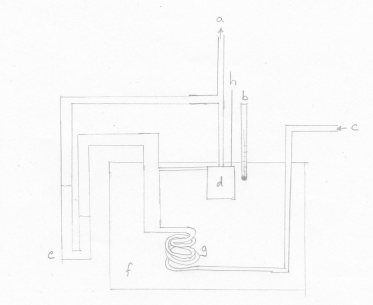
\includegraphics[scale=1.2]{VersuchsaufbauJT.png} \end{center}
\caption{Versuchsaufbau.}
\end{figure}
\FloatBarrier

a)Gasanschluss\\
b)Thermometer\\
c)Gaseinlass\\
d)Drosselstelle\\
e)Differenzdruckmanometer\\
f)Wärmebad\\
g)Wärmetauscher\\
h)$\Delta$T-Messstelle\\

\section{Durchführung}
Ziel des Versuches war die Bestimmung der Temperaturabhängigkeit des Joule-Thompson-Koeffizienten $\mu_\mathrm{JT}$ von $\mathrm{N}_2$ und $\mathrm{CO}_2$. Dabei wurde das jeweilige Gas isenthalp durch eine Drosselstelle expandiert und dabei Druck- und Temperaturänderung notiert.\\

Zu Beginn wurde eine Druckdifferenz von 0.1 atm eingestellt und das Temperaturdifferenz -Messgerät auf 0 geeicht. 
In 0.2 atm Druckdifferenz-Schritten wurde bis zur einer Druckdifferenz von 1.7 atm erhöht und die Temperaturdifferenz jeweils nach 10 Sekunden Wartezeit notiert. Bei 1.7 atm wurde um 0.5 atm erhöht und die Temperatur gemessen. Von 1.75 atm wurde in 0.2 atm Schritten die Druckdifferenz erniedrigt und die Temperaturdifferenz notiert. Dieser Messvorgang wurde mit Stickstoff und Kohlenstoffdioxidgas bei Zimmertemperatur, dann bei 0~°C und zu letzt bei 50~°C durchgeführt.
\chapter{Auswertung}

%Darstellung und Auswertung der Messergebnisse
%Fehlerrechnung und Fehlerdiskussion (statistische und systematische fehler)
%Abschätzung systematischer Fehler
%Endergebnis mit Fehlerangabe


\section{Berechnung des mitteleren Joule-Thomson-Koeffizienten}
Der mittlere Joule-Thompson-Koeffizient entspricht der Steigung bei einer Auftragung von $\Delta T$ gegen $\Delta p$. Hierbei wird der Differentialquotient durch einen Differenzenquotienten ersetzt.\\

\begin{equation}
\mu_\mathrm{JT} = \left(\frac{\partial T}{\partial p}\right)_H
\end{equation}

Die sich ergebenden Steigungen sind in nachfolgender Tabelle aufgelistet. Die Fehler wurden als Standardfehler der Auftragung berechnet. Die einzelnen Auftragungen sind im Anhang zu finden.\\

\begin{table} [h]
\centering
\caption{Experimentell bestimmt Joule-Thomson-Koeffizienten $\mu_{\text{JT, exp.}}$}
\begin{tabular} {l | c|  c}
	 &  $T$ [K] & $\langle \mu_{\text{JT, exp.}} \rangle$/~$\frac{\mathrm{K}}{\mathrm{bar}}$ \\
	 \hline
	  $CO_\mathrm{2}$ & 273.25 & 1.20 $\pm$ 0.04 \\
	   & 295.95 & 1.01 $\pm$ 0.06\\
	  & 323.95 & 0.710 $\pm$ 0.05\\
	\hline
	$N_2$ & 273.25 & 0.181  $\pm$  0.02\\
	& 295.95 & 0.175 $\pm$ 0.02\\
	& 323.95& 0.120 $\pm$ 0.01\\
\end{tabular}
\end{table}
\section{Herleitung $c_v^\mathrm{ vib}$}

Zur Berechnung von $\mu_\mathrm{JT}$ wird neben tabellierten Größen vor allem die molare Wärmekapazität bei konstantem Druck $c_p$ benötigt. Diese wiederum ergibt sich aus der molaren Wärmekapazität bei konstantem Volumen $c_V$:

\begin{equation}
c_p = c_V +R \label{cpauscv}
\end{equation}

Da Wärme in Form von Schwingungsenergie (Vibration), Rotationsenergie und Bewegungsenergie (Translation) von einzelnen Molekülen aufgenommen und somit gespeichert werden kann, liefern diese je ihren Beitrag zur molaren Wärmekapazität (die Energieaufnahme in Form von Elektronenanregung spielt in diesem Fall keine Rolle und wird daher vernachlässigt):

\begin{equation}
c_V = c_V^\mathrm{ vib} + c_V^\mathrm{ rot} + c_V^\mathrm{trans}  
\label{cv=rotvibtrans}
\end{equation}

Die einzelnen Beiträge ergeben sich je aus den Freiheitsgraden für Moleküle, wobei jedes Molekül $3N$ Freiheitsgrade hat. Die sind je nach Atomzahl und Geometrie (linear/gewinkelt) unterschiedlich. Für lineare Moleküle (2 Rotationsfreiheitsgrade) verbleiben noch $3N-5$ Schwingungsfreiheitsgrade. \\
Translations- und Rotationsfreiheitsgrade steuern je $\frac{1}{2} R$ zu $c_V$ hinzu; da die Vibration in potentielle und kinetische Energie aufteilbar ist steuert jeder Vibrationsfreiheitsgrad $1R$ zur Wärmekapazität bei. So ergeben sich $U$ und $c_V$ (Tabelle \ref{cvtabelle})\\.

 \begin{equation}
 U= \frac{1}{2} \cdot f \cdot Nk_\mathrm{B}T
 \end{equation}

\begin{equation}
c_V = \left(\frac{\partial U}{\partial T}\right)_V =\frac{1}{2} \cdot f \cdot N k_\mathrm{B} = \frac{1}{2}\cdot f\cdot R
\end{equation}



\begin{table} [h] \label{cvtabelle}
\centering
\caption{$\text{c}_v$-Wert der Translations, Rotation und Schwingung von $\text{N}_2$ und $\text{CO}_2$.}
\begin{tabular} {l | c|  c | c}
	 & $c_V^\mathrm{ vib}$  & $c_V^\mathrm{ rot}$ & $c_V^\mathrm{trans}$\\
	 \hline
	 $N_2$ & $R$ & $R$ &$\frac{3}{2}R$\\
	  $CO_2$ & 4$R$ & $R$ &$\frac{3}{2}R$\\
\end{tabular}
\end{table}

Da die Schwingung erst bei sehr hohen Temperaturen vollständig angeregt ist, muss folgende Formel verwendet werden, die hier hergeleitet wird: \\


\begin{equation}
c_V^\mathrm{ vib} = R\cdot(hv\beta)^2 \frac{\mathrm{exp}(hv\beta)}{\mathrm{exp}(hv\beta -1)^2} \label{cvviblangeFormel}
\end{equation}


mit $\beta=\frac{1}{k_\mathrm{B} \cdot T}$.\\

Grundlage bildet die Vibrationszustandssumme des Systems:\\

\begin{equation}
Z_\mathrm{vib}= \left[\frac{\mathrm{exp}(-\frac{hv}{2k_\mathrm{B}T})}{1-\mathrm{exp}(-\frac{hv}{k_\mathrm{B}T})}\right]^N
\end{equation}

Bei adiabatischer Prozessführung ist die Wärmezufuhr/-abgabe gleich der Änderung der inneren Energie. Die Vibrationszustandssumme steht mit letzterer folgendermaßen im Zusammenhang:\\

\begin{equation}
U_\mathrm{vib}= -k_\mathrm{B}T^2 \frac{\partial \mathrm{ln}Z_\mathrm{vib}}{\partial T} = N\frac{hv}{2} +\frac{Nhv}{\mathrm{exp}\left(\frac{hv}{k_\mathrm{B}T}\right)-1}= U_\mathrm{m}^\mathrm{vib} = R \Theta \left[ \frac{1}{2} + \frac{1}{\mathrm{exp}(\frac{\Theta_\mathrm{vib}}{T}) -1}\right]
\end{equation}

Mit\\

\begin{equation}
\Theta_\mathrm{vib} = \frac{hv}{k_\mathrm{B}}
\end{equation}


Die Ableitung der molaren inneren Energie ergibt die molare Wärmekapazität:\\


\begin{equation}
c_V = \frac{\partial U_\mathrm{m}}{\partial T}\bigg \vert_\mathrm{V}
\end{equation}

Analog gilt:

\begin{equation}
c_V^\mathrm{vib} = \frac{\delta U_\mathrm{m}^\mathrm{vib}}{\delta T}\bigg \vert_\mathrm{V}
\end{equation}

Das ganze abgeleitet ergibt wiederum $c_v^{vib}$ als herzuleitende Formel.\\


\section{Berechnung von $\mu_\mathrm{JT}$ aus der Virialgleichung}

Der Unterschied eines realen Gases zum idealen Gas wird mittels Virialentwicklung beschrieben, wobei hier ein Abbruch nach dem 2. Virialkoeffizienten stattfindet.\\

\begin{equation}
pV_\mathrm{m} = RT + B(T) \cdot p \label{Virialgleichung}
\end{equation}

Wie in Gleichung (\ref{Virialgleichung}) gut zu sehen ist, bildet der 2. Virialkoeffizient einen linearen Korrekturterm für den Druck im Bezug zum idealen Gasgesetz.
Der Joule-Thomson-Koeffizient kann in Abhängigkeit des 2. Virialkoeffizienten folgendermaßen ausgedrückt werden:

\begin{equation}
\mu_\mathrm{JT} = \frac{1}{c_p}\left( T \frac{\partial B}{\partial T} \bigg \vert_p - B\right)
\end{equation}

Hier wird mit der reduzierten Temperatur gerechnet (Gleichung \ref{reduzierteTemperatur} ). 

\begin{equation}
T^* = \frac{T}{\varepsilon} \label{reduzierteTemperatur}
\end{equation}

$\varepsilon$ ist dabei die Lennard-Jones- Potentialtiefe in der Einheit Kelvin. $B(T)$ hängt mit $B^*(T)$ zusammen (Gleichung \ref{Zsh.BB*} ).\\

\begin{equation}
B(T) = b_0 \cdot B^*(T^*) = \frac{2}{3} \cdot \pi N_\mathrm{L} \sigma^3 \cdot B^*(T^*) \label{Zsh.BB*}
\end{equation}

Somit wird $\mu_\mathrm{JT}$ letztendlich folgendermaßen berechnet:\\

\begin{equation} \label{EndgleichungJT}
\mu_\mathrm{JT} = \frac{1}{c_p}\left(b_0 \cdot T^* \frac{\partial B^*(T^*)}{\partial T^*} \bigg \vert_\mathrm{p} - b_0 \cdot B^*(T^*)\right)
\end{equation}


Die Rechnung liefert die theoretischen Werte der Joule-Thomson-Koeffizienten zu den gemessenen Temperaturen. Alle anderen Größen der Rechnung wurden dem Praktikumsskript entnommen, auch $B^*(T^*)$ und $T^*\frac{dB^*(T^*)}{dT^*}$ pro $T^*$\protect\footnote{Hirschfelder, Curtiss, Bird, New Yorck 1954}. Für die Rechnung müssen die Kreisfrequenzen $\omega$ aus dem Praktikumsskript in Schwingungsfrequenzen $\nu$ umgerechnet werden (Gleichung (\ref{KreisfrequenzUmrechnung})). Die Werte sind in Tabelle (\ref{TabelleSchwingungsfrequenzen}) dargestellt.  \\

\begin{equation}
\nu = \omega \cdot \mathrm{c} \label{KreisfrequenzUmrechnung}
\end{equation}


\begin{table}\caption{Schwingungsfrequenzen} \label{TabelleSchwingungsfrequenzen}
\begin{tabular}{r|r|r|r} 
& $\nu_{1}$ [$ 10^{13} \cdot \text{s}^{-1}$]& $\nu_{2/3} [10^{13} \cdot \text{s}^{-1}$]& $\nu_{4}$ [$ 10^{13} \cdot \text{s}^{-1}$]\\
\hline
$N_2$&7,086&-&-\\
$CO_2$& 4,026&	2,001&7,043\\
\end{tabular}
\end{table}


Da $CO_2$ 4 Schwingungsfreiheitsgrade besitzt, wurde $c_V^\mathrm{ vib}$ für jede Schwingung berechnet und die Werte summiert. Einsetzen in Gleichung (\ref{cvviblangeFormel}) und (\ref{cv=rotvibtrans}) liefert die Ergebnisse aus Tabelle (\ref{cvvibundcvTabelle}).\\

\begin{table}\caption{$c_V^\mathrm{vib}$ und $c_V$} \label{cvvibundcvTabelle}
\begin{tabular}{r|r|c|c|c|r|r}
&$T$[K]& \multicolumn{3}{|r|}{$c_V^\mathrm{vib}$ [$\frac{\mathrm{J}}{\mathrm{K}\cdot \mathrm{mol}}$] }&$c_V^\mathrm{vib}$ [$\frac{\mathrm{J}}{\mathrm{K}\cdot \mathrm{mol}}$] & $ c_V$ [$\frac{\mathrm{K}}{\mathrm{bar}}$] \\
&&$\nu_{1}$&$\nu_{2} = \nu_{3}$&$\nu_{4}$&gesamt&\\
\hline

	  $\text{N}_\mathrm{2}$ & 273,3&  0,005206&-& - &  0,005206 &20,79\\
	   & 295.9  &0,01146&-&-& 0,01146 &20,80\\
	  & 324,0 &0,02585 &-&-& 0,02585 & 20,81\\
\hline  
$CO_2$&273,3&0,3538&	3,248&	0,005399&6,856&27,64\\
&296,1&0,5194&	3,696&	0,01189&7,922&28,71\\
&324,0& 0,7638&	4,192&	0,02663&9,174&29,96\\
\end{tabular}
\end{table}
\FloatBarrier

Durch Einsetzen in Gleichung (\ref{cpauscv}) und (\ref{EndgleichungJT}) ergeben sich für $c_p$ und~$<~\mu_{\text{JT}}^{\text{Th.}}>$ folgende Werte :\\

\begin{table} [h]
\centering
\caption{Theoretisch bestimmte Joule-Thomson-Koeffizienten $\langle \mu_{\text{JT, th.}} \rangle$ für $\text{N}_2$  und $CO_2$.}
\begin{tabular} {l | c|  c | c}
	 &  $T$ [K] &  $c_p$ [$\frac{\mathrm{J}}{\mathrm{K}\cdot \mathrm{mol}}$] & $ <\mu_{\text{JT}}^{\text{th.}}>$ [$\frac{\mathrm{K}}{\mathrm{bar}}$] \\
	 \hline
	  $\text{N}_\mathrm{2}$ & 273.25 & 29,11 & 0,0396\\
	   & 295.95 & 29,11 & 0,0345\\
	  & 323.95 & 29,13 & 0,0272 \\
	\hline
	$CO_2$ & 273.25& 35,96&0,106  \\
	& 295.95 & 37,02& 0,0926\\
	& 323.95& 38,28& 0,0771\\
\end{tabular}
\end{table}
\FloatBarrier


\section{Fehlerrechnung}
Die Ungenauigkeit der Auftragung wurde mittels der Funktion \textit{Linear Fit} des Programms \textit{Origin 8.5G} bestimmt. Es wurde die Standerabweichung genutzt. \\
Die Ungenauigkeit der $\mu_{\text{JT}}^{\text{th.}}$ wurden nicht bestimmt, da dieser Wert aus Literaturwerten bestimmt wurde.
%\subsection{Vergleich mit den Literaturwerten}
%Für die Molmasse der Substanz im Cyclohexan ergeben sich folgende Werte:\\
%$M_A = (13 \cdot 10 \pm 3 \cdot 10){~} \mathrm{g{~}mol^{-1}}$\\\\
%$M_B = (12 \cdot 10 \pm 2 \cdot 10){~} \mathrm{g{~}mol^{-1}}$\\\\
%Dabei handelt es sich um Campher, dieses hat eine Molmasse von $ 152,23{~} \mathrm{g{~}mol^{-1}}$ \footnote{https://de.wikipedia.org/wiki/Campher abgerufen am \textbf{13.12.2015}} Beide Werte weichen um $15-21\%$ nach unten hin ab, dies legt einen systematischen Fehler nahe, wobei der Wert 1 noch im Fehlerintervall liegt.\\\\
%Für die Molmasse der im Wasser gelösten Substanz ergibt sich:\\\\
%$M_A = (6 \cdot 10 \pm 3 \cdot 10){~} \mathrm{g{~}mol^{-1}}$\\\\
%$M_B = (5\cdot 10 \pm 3\cdot 10 ){~} \mathrm{g{~}mol^{-1}}$\\\\
%Es handelt sich bei der im Wasser gelösten Substanz um Kaliumchlorid, dieses hat eine Molmasse von $74,55{~} \mathrm{g{~}mol^{-1}}$ {~}\footnote{https://de.wikipedia.org/wiki/Kaliumchlorid abgerufen am \textbf{09.12.2015}} Die starke Abweichung von $20-30\%$ der Werte lässt sich nicht mithilfe der Fehlerfortpflanzung erklären, daher muss es sich um systematische Fehler handeln. 
\chapter{Diskussion}
Die Auswertungsergebnisse und die Literaturwerte sind in Tabelle \ref{TabelleEndeN2} und Tabelle \ref{TabelleEndeCO2} dargestellt. \\


\begin{table}[h]
\centering
\caption{Werte des Joule-Thomson-Koeffizienten für $\text{N}_2$.}
\begin{scriptsize}
\begin{tabular}{c|c|c|c} \label{TabelleEndeN2}
Temperatur/~°C&$ \mu_{\text{N$_{2}$,exp.}}$/~$\frac{\text{K}}{\text{bar}}$&$ \mu_{\text{N$_{2}$,th.}}$/~$\frac{\text{K}}{\text{bar}}$&$ \mu_{\text{N$_{2}$,Lit.}}$/~$\frac{\text{K}}{\text{bar}}$\\
\hline
0,1 & 0,181 $\pm$ 0,02& 0,252 &0,26$^1$\\
\hline
22,7 & 0,175 $\pm$ 0,02& 0,220&0,25$^2$\\
\hline
50,8& 0,120 $\pm$ 0,01& 0,173&0,19$^1$\\
\end{tabular}
\end{scriptsize}
\end{table}
\noindent
\FloatBarrier


\begin{table}[h]
\centering
\caption{Werte des Joule-Thomson-Koeffizienten für $\text{CO}_2$.}
\begin{scriptsize}
\begin{tabular}{c|c|c|c} \label{TabelleEndeCO2}
Temperatur/~°C&$ \mu_{\text{CO$_{2}$,exp.}}$/~$\frac{\text{K}}{\text{bar}}$&$ \mu_{\text{CO$_{2}$,th.}}$/~$\frac{\text{K}}{\text{bar}}$&$ \mu_{\text{CO$_{2}$,Lit.}}$/~$\frac{\text{K}}{\text{bar}}$\\
\hline
0,1 & 1,20 $\pm$ 0,04& 1,21&1,31$^1$\\
\hline
22,8 & 1,01 $\pm$ 0,06& 1,05&1,12$^2$\\
\hline
50,8& 0,710 $\pm$ 0,05& 0,878&0,91$^1$\\
\end{tabular}
\end{scriptsize}
\end{table}
\noindent
\FloatBarrier

\footnotetext{ $^1$Atkins, P.W.: \emph{Physikalische Chemie}, Wiley-VCH, Weinheim, \textbf{2006}.}
\footnotetext{$^2$Zemansky: \emph{Heat and Thermodynamics}, Mc Graw-Hill, New York, \textbf{1990}.}


Die theoretisch ermittelten Joule-Thomson-Koeffizienten für $N_2$ liegen nicht innerhalb der Fehlergrenzen der experimentell ermittelten Werte und haben alle eine positive Abweichung. Die Abweichung der Literaturwerte zu den theoretischen Werten dagegen ist ebenfalls positiv, aber nicht ganz so groß. \\

Für $CO_2$ ist die Messung anscheinend deutlich genauer verlaufen; die theoretischen Werte liegen bis auf den letzten Wert innerhalb der Fehlergrenzen und auch die Abweichung zu den Literaturwerten ist deutlich geringer. Allerdings muss der Vergleich auch mit Vorsicht erfolgen, da die Temperaturen nicht ganz übereinstimmen.\\

Für $N_2$ sind die Fehlergrenzen auf jeden Fall zu klein bzw. die Messung zu ungenau. Ein zu geringer Wert bedeutet, dass die gemessene Temperaturänderung zu klein oder die Druckänderung zu groß war. Das kann auf schlechte Isolierung zurückzuführen sein. Undichtigkeit der Apparatur ist eher unwahrscheinlich; sonst wären die Werte zu groß. Auffällig ist dennoch bei den Auftragungen die starke Streuung der Werte und der dennoch kleine Fehler. Bei $N_2$ ist die Streuung deutlich größer. Durch die schwankenden Temperaturwerte und die abnehmende Druckdifferenz war die Messung außerdem sehr ungenau.\\
  
Die Abweichung der theoretischen Joule-Thomson-Koeffizienten von den Literaturwerten ist weniger stark. Hier wurde auch lediglich mit einer fehlerbehafteten Größe gerechnet, der Temperatur. Der Fehler war relativ gering, wurde jedoch durch das tabellarische Ablesen der zu $T^*$ zugehörigen $B^*$ und $T^* \cdot \frac{\partial B^*(T^*)}{\partial T^*}$-Werte deutlich verfälscht. Am Schluss wurde das Ergebnis auf 3 signifikante Stellen angegeben, allerdings konnte nur mit Werten gerechnet werden, die $T^*$ ungefähr entsprechen. An dieser Stelle wäre es sinnvoller, eine Formel zur Berechnung der zugehörigen $B^*$ und $T^* \cdot \frac{\partial B^*(T^*)}{\partial T^*}$-Werte zu verwenden.\\

Der Joule-Thomson-Koeffizient ist für ideale Gase $=0$ und demnach leichter zu bestimmen, je mehr die Gase vom idealen Verhalten abweichen. Wahrscheinlich sind die Werte von $N_2$ so unterschiedlich, da es sich aufgrund der geringeren Masse und unpolaren Bindung im Gegensatz zu $CO_2$ eher ideal verhält und die Messung sehr sensibel ist; dh. sich Störfaktoren viel stärker auswirken als bei $CO_2$. Dies ist auch daran erkennbar, dass $\mu_\mathrm{JT}$ für $N_2$ viel kleiner, d.h. viel näher am idealen Verhalten "0" ist als $\mu_\mathrm{JT}$ für $CO_2$.\\
Bei beiden Gasen sinkt $\mu_\mathrm{JT}$ auch mit steigender Temperatur, d.h. durch die ohnehin schon schnellere Bewegung der Teilchen ist die Abweichung vom idealen Verhalten geringer und auch die Temperaturabsinkung bei Expandieren geringer.\\
 Außerdem kann auch infrage gestellt werden, inwieweit diese Messmethode sinnvoll ist. Dadurch, dass der Differenzialquotient zu einem Differenzenquotienten integriert wird, wird zur Berechnung angenommen, dass $\mu_\mathrm{JT}$ nur temperaturabhängig ist, dh. die Temperaturänderung pro Druckänderung immer dieselbe. Besonders bei den $N_2$-Auftragungen wird deutlich, dass diese Näherung zu groß ist.\\ 
 
\chapter{Anhang}
\begin{center}
\begin{figure}[h]
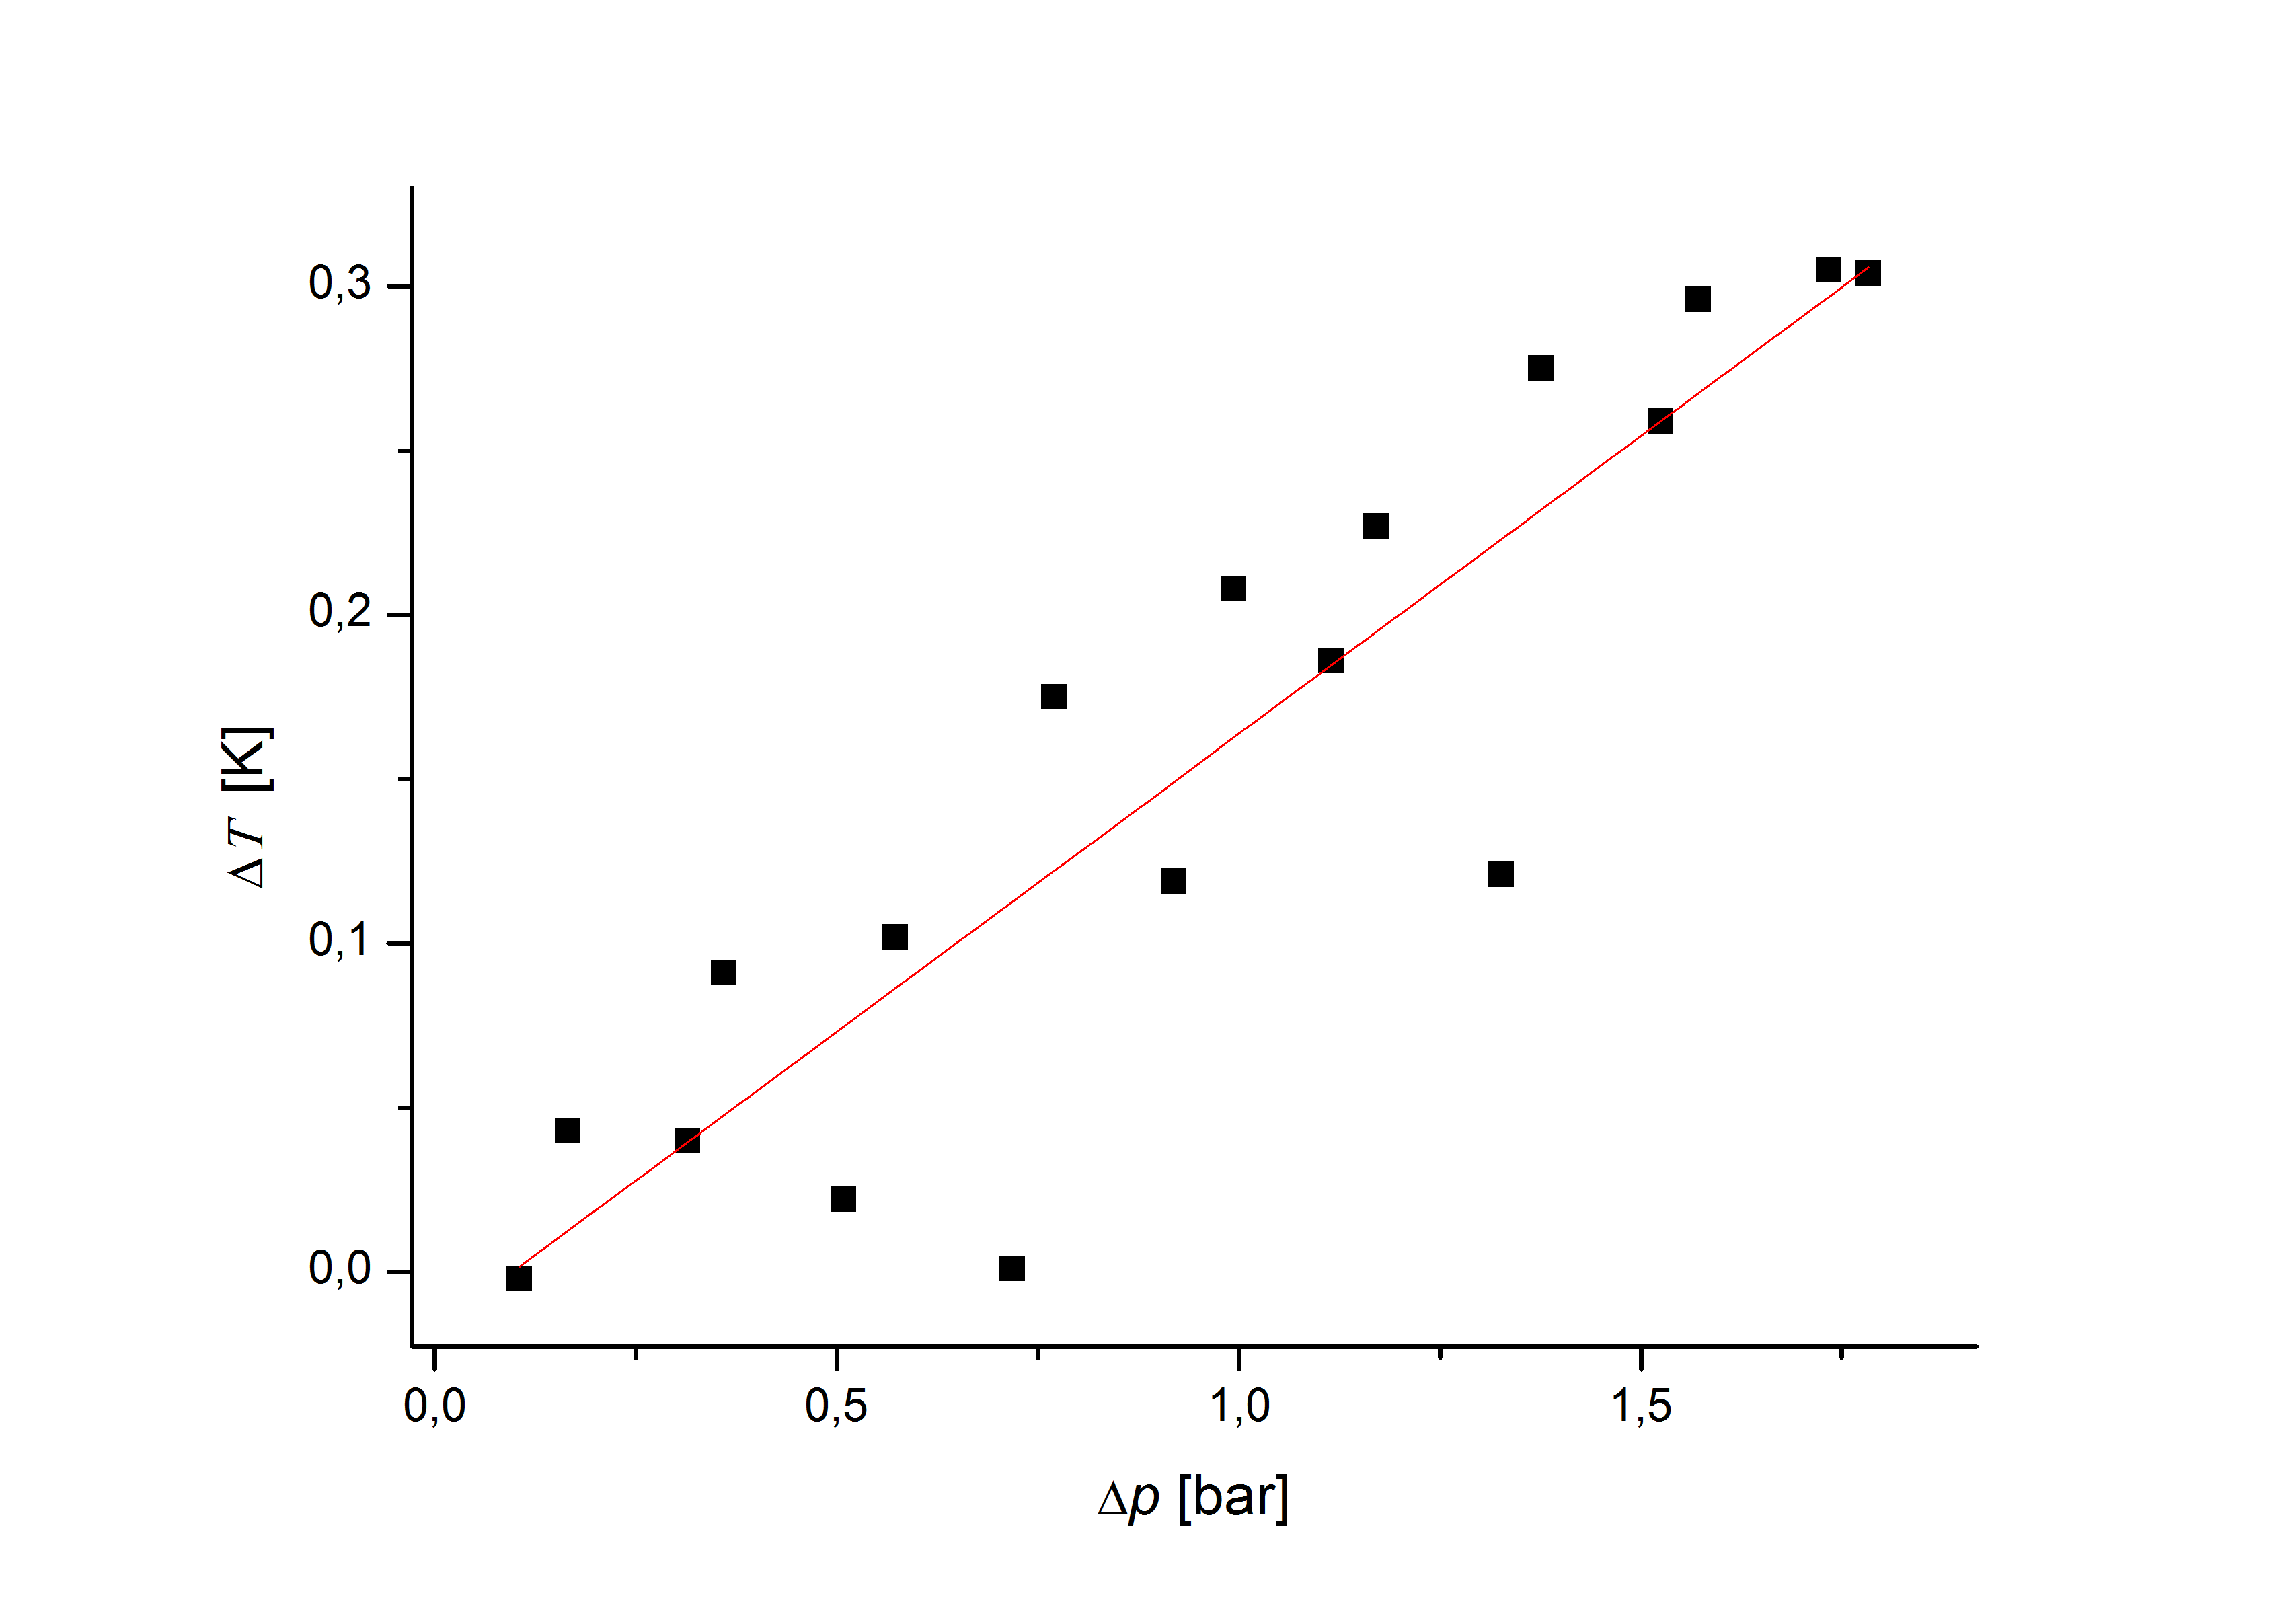
\includegraphics[width=13.5cm]{N2bei0Grad.png}
\caption{$N_2$ bei 0,1~°C.}
\end{figure}
\end{center}
\begin{center}
\begin{figure}[h]
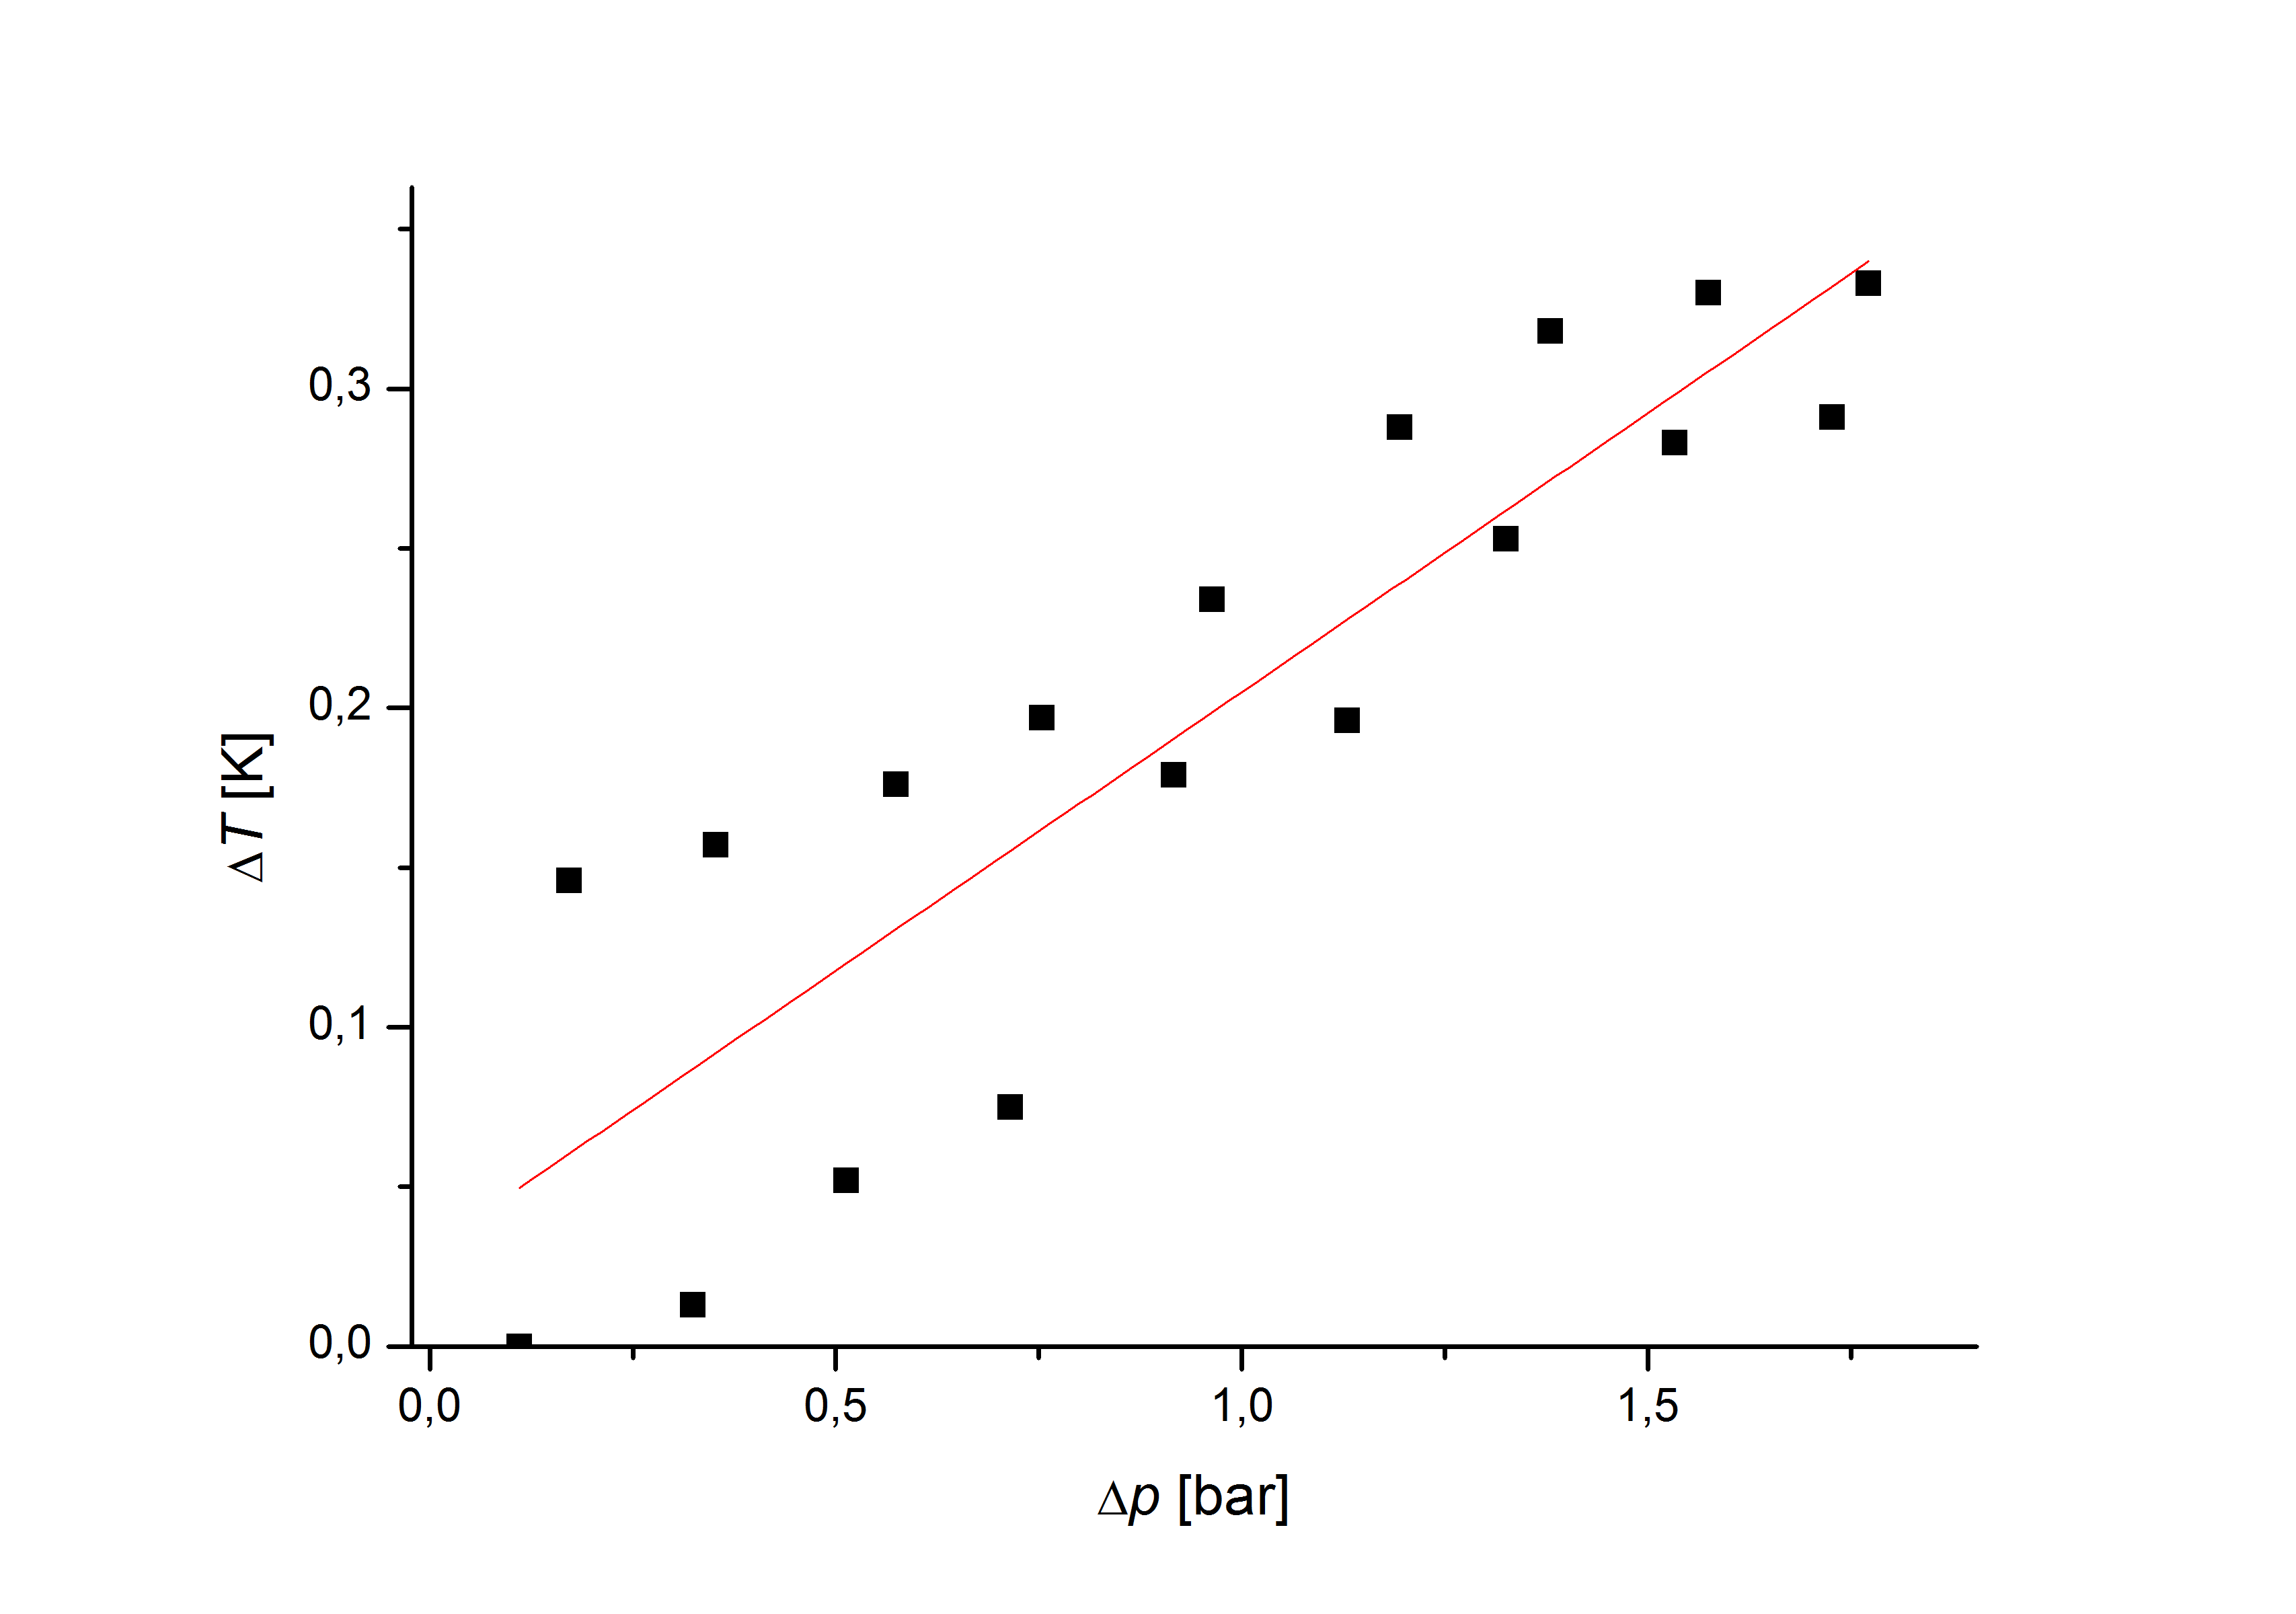
\includegraphics[width=13.5cm]{N2bei22,7.png}
\caption{$N_2$ bei 22,7~°C.}
\end{figure}
\end{center}
\begin{center}
\begin{figure}[h]
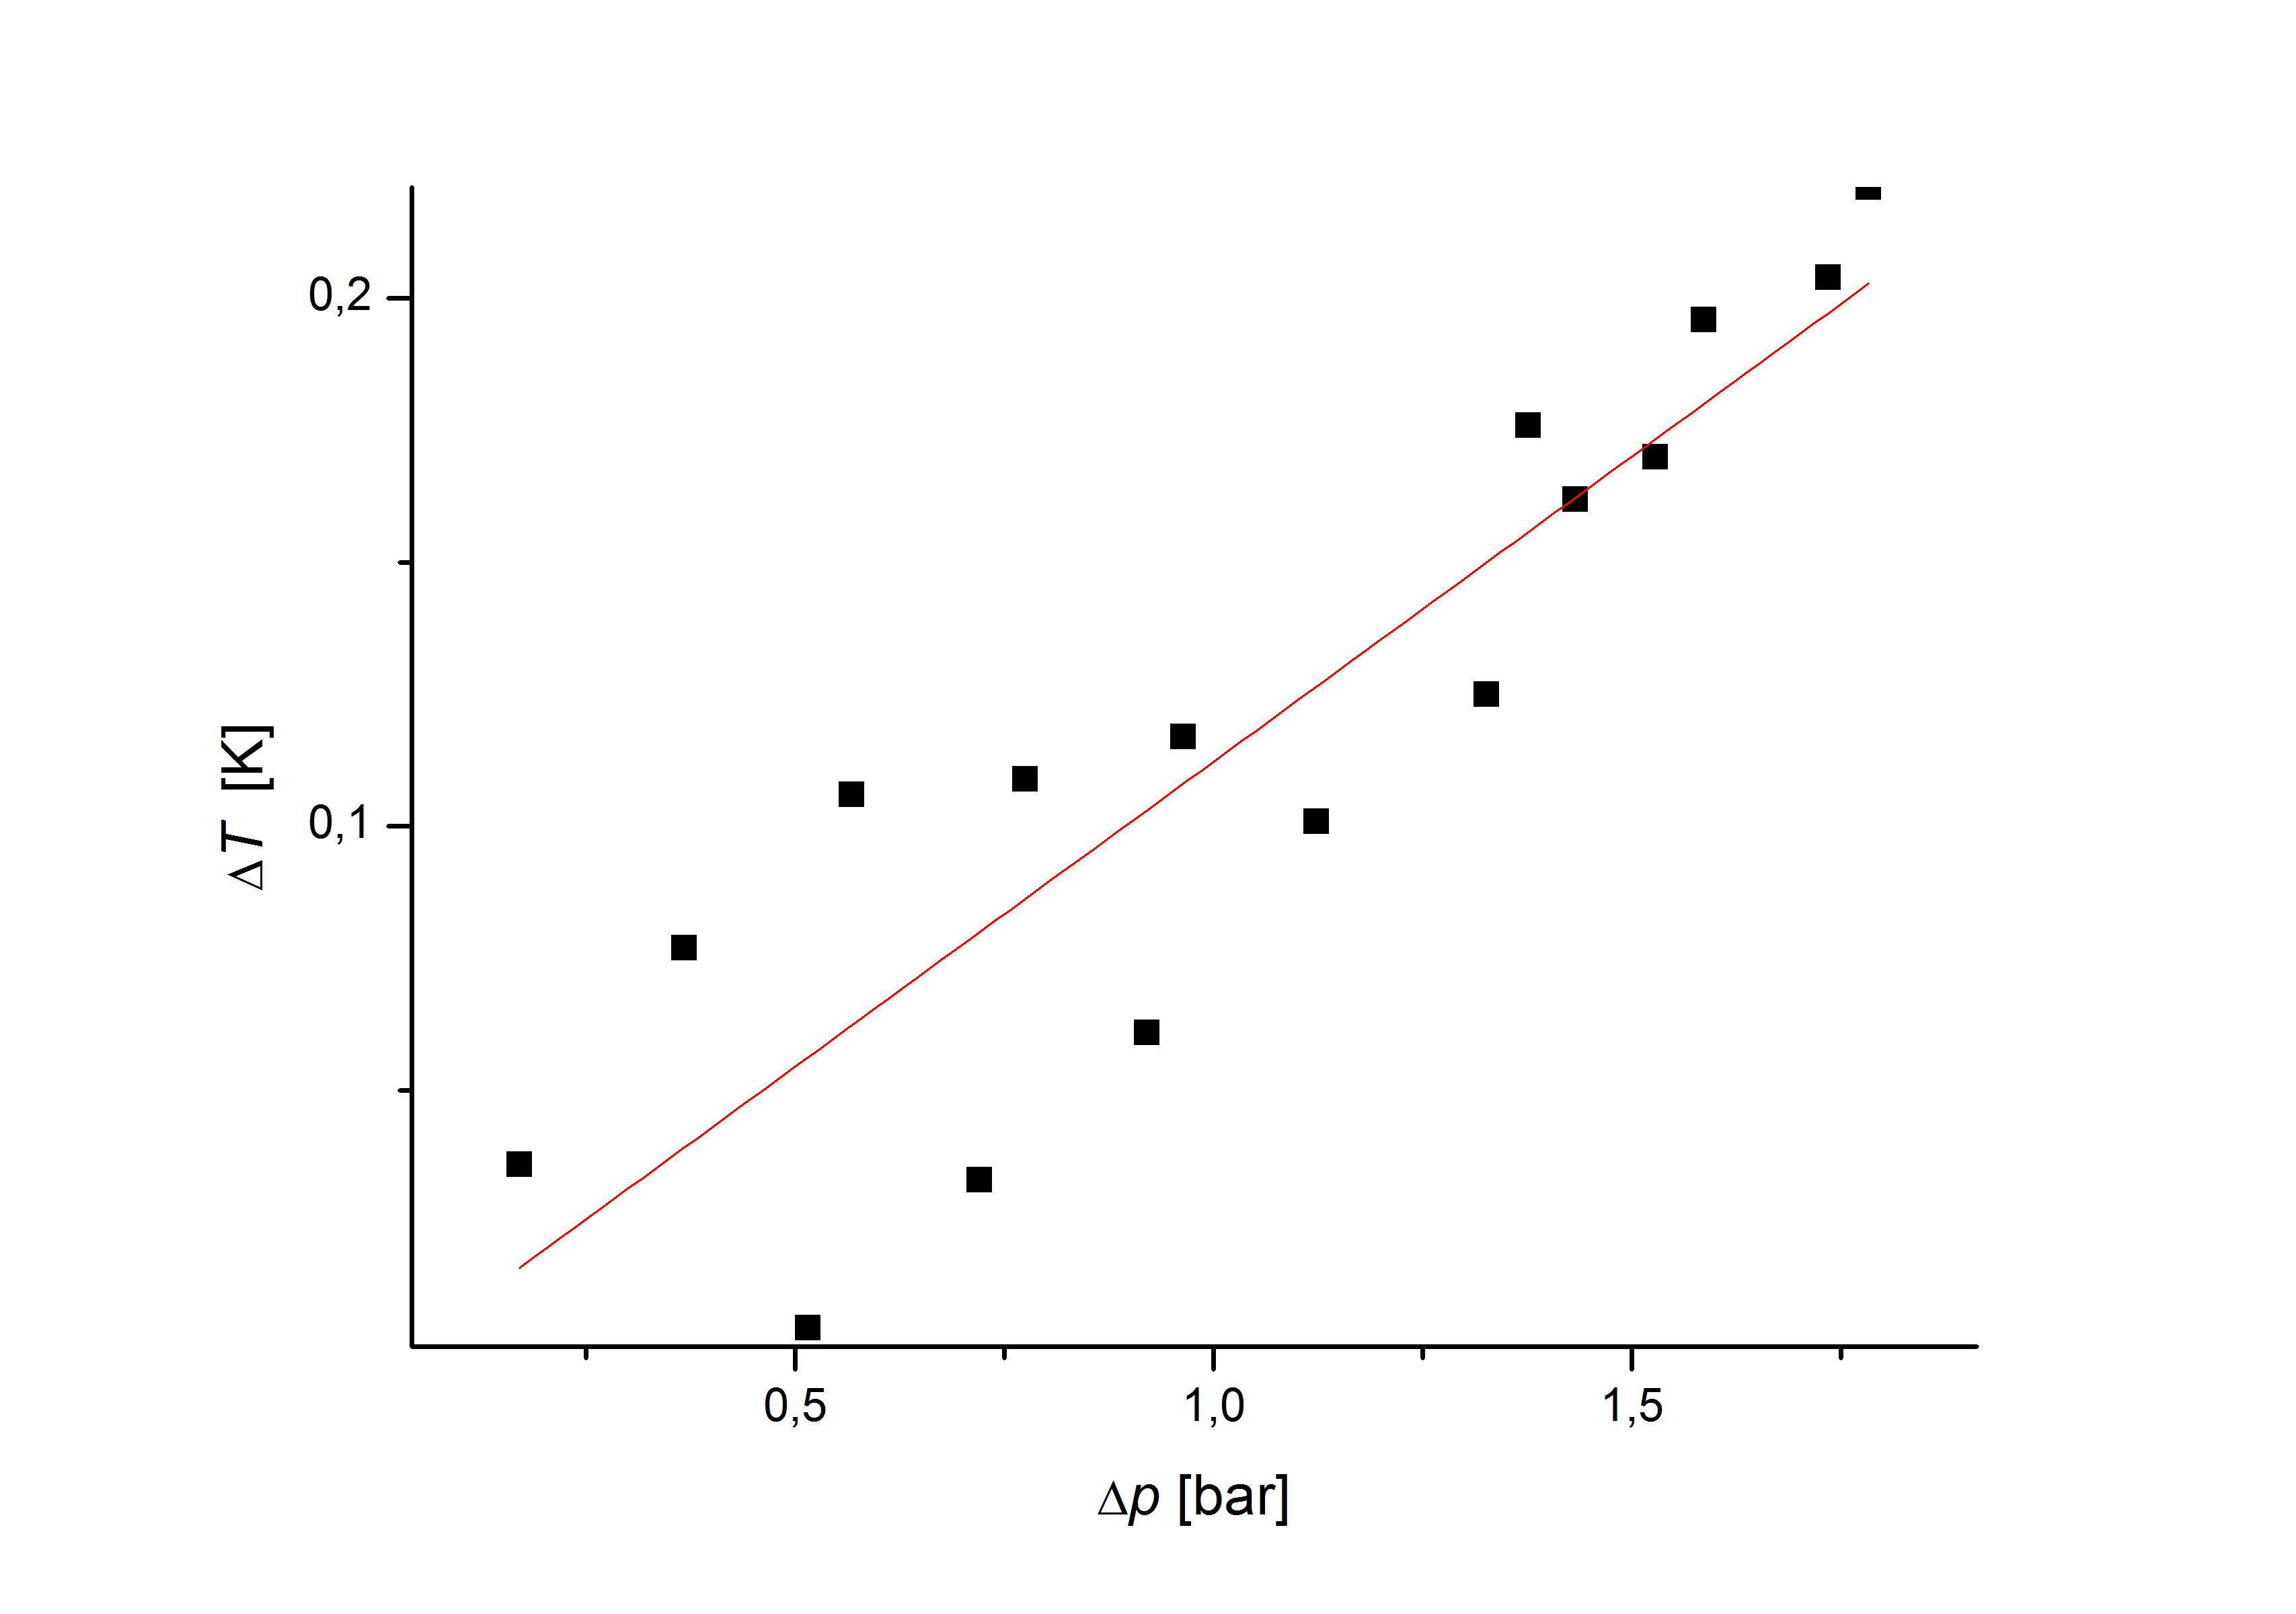
\includegraphics[width=13.5cm]{N2bei50.png}
\caption{$N_2$ bei 50,8~°C.}
\end{figure}
\end{center}
\begin{center}
\begin{figure}[h]
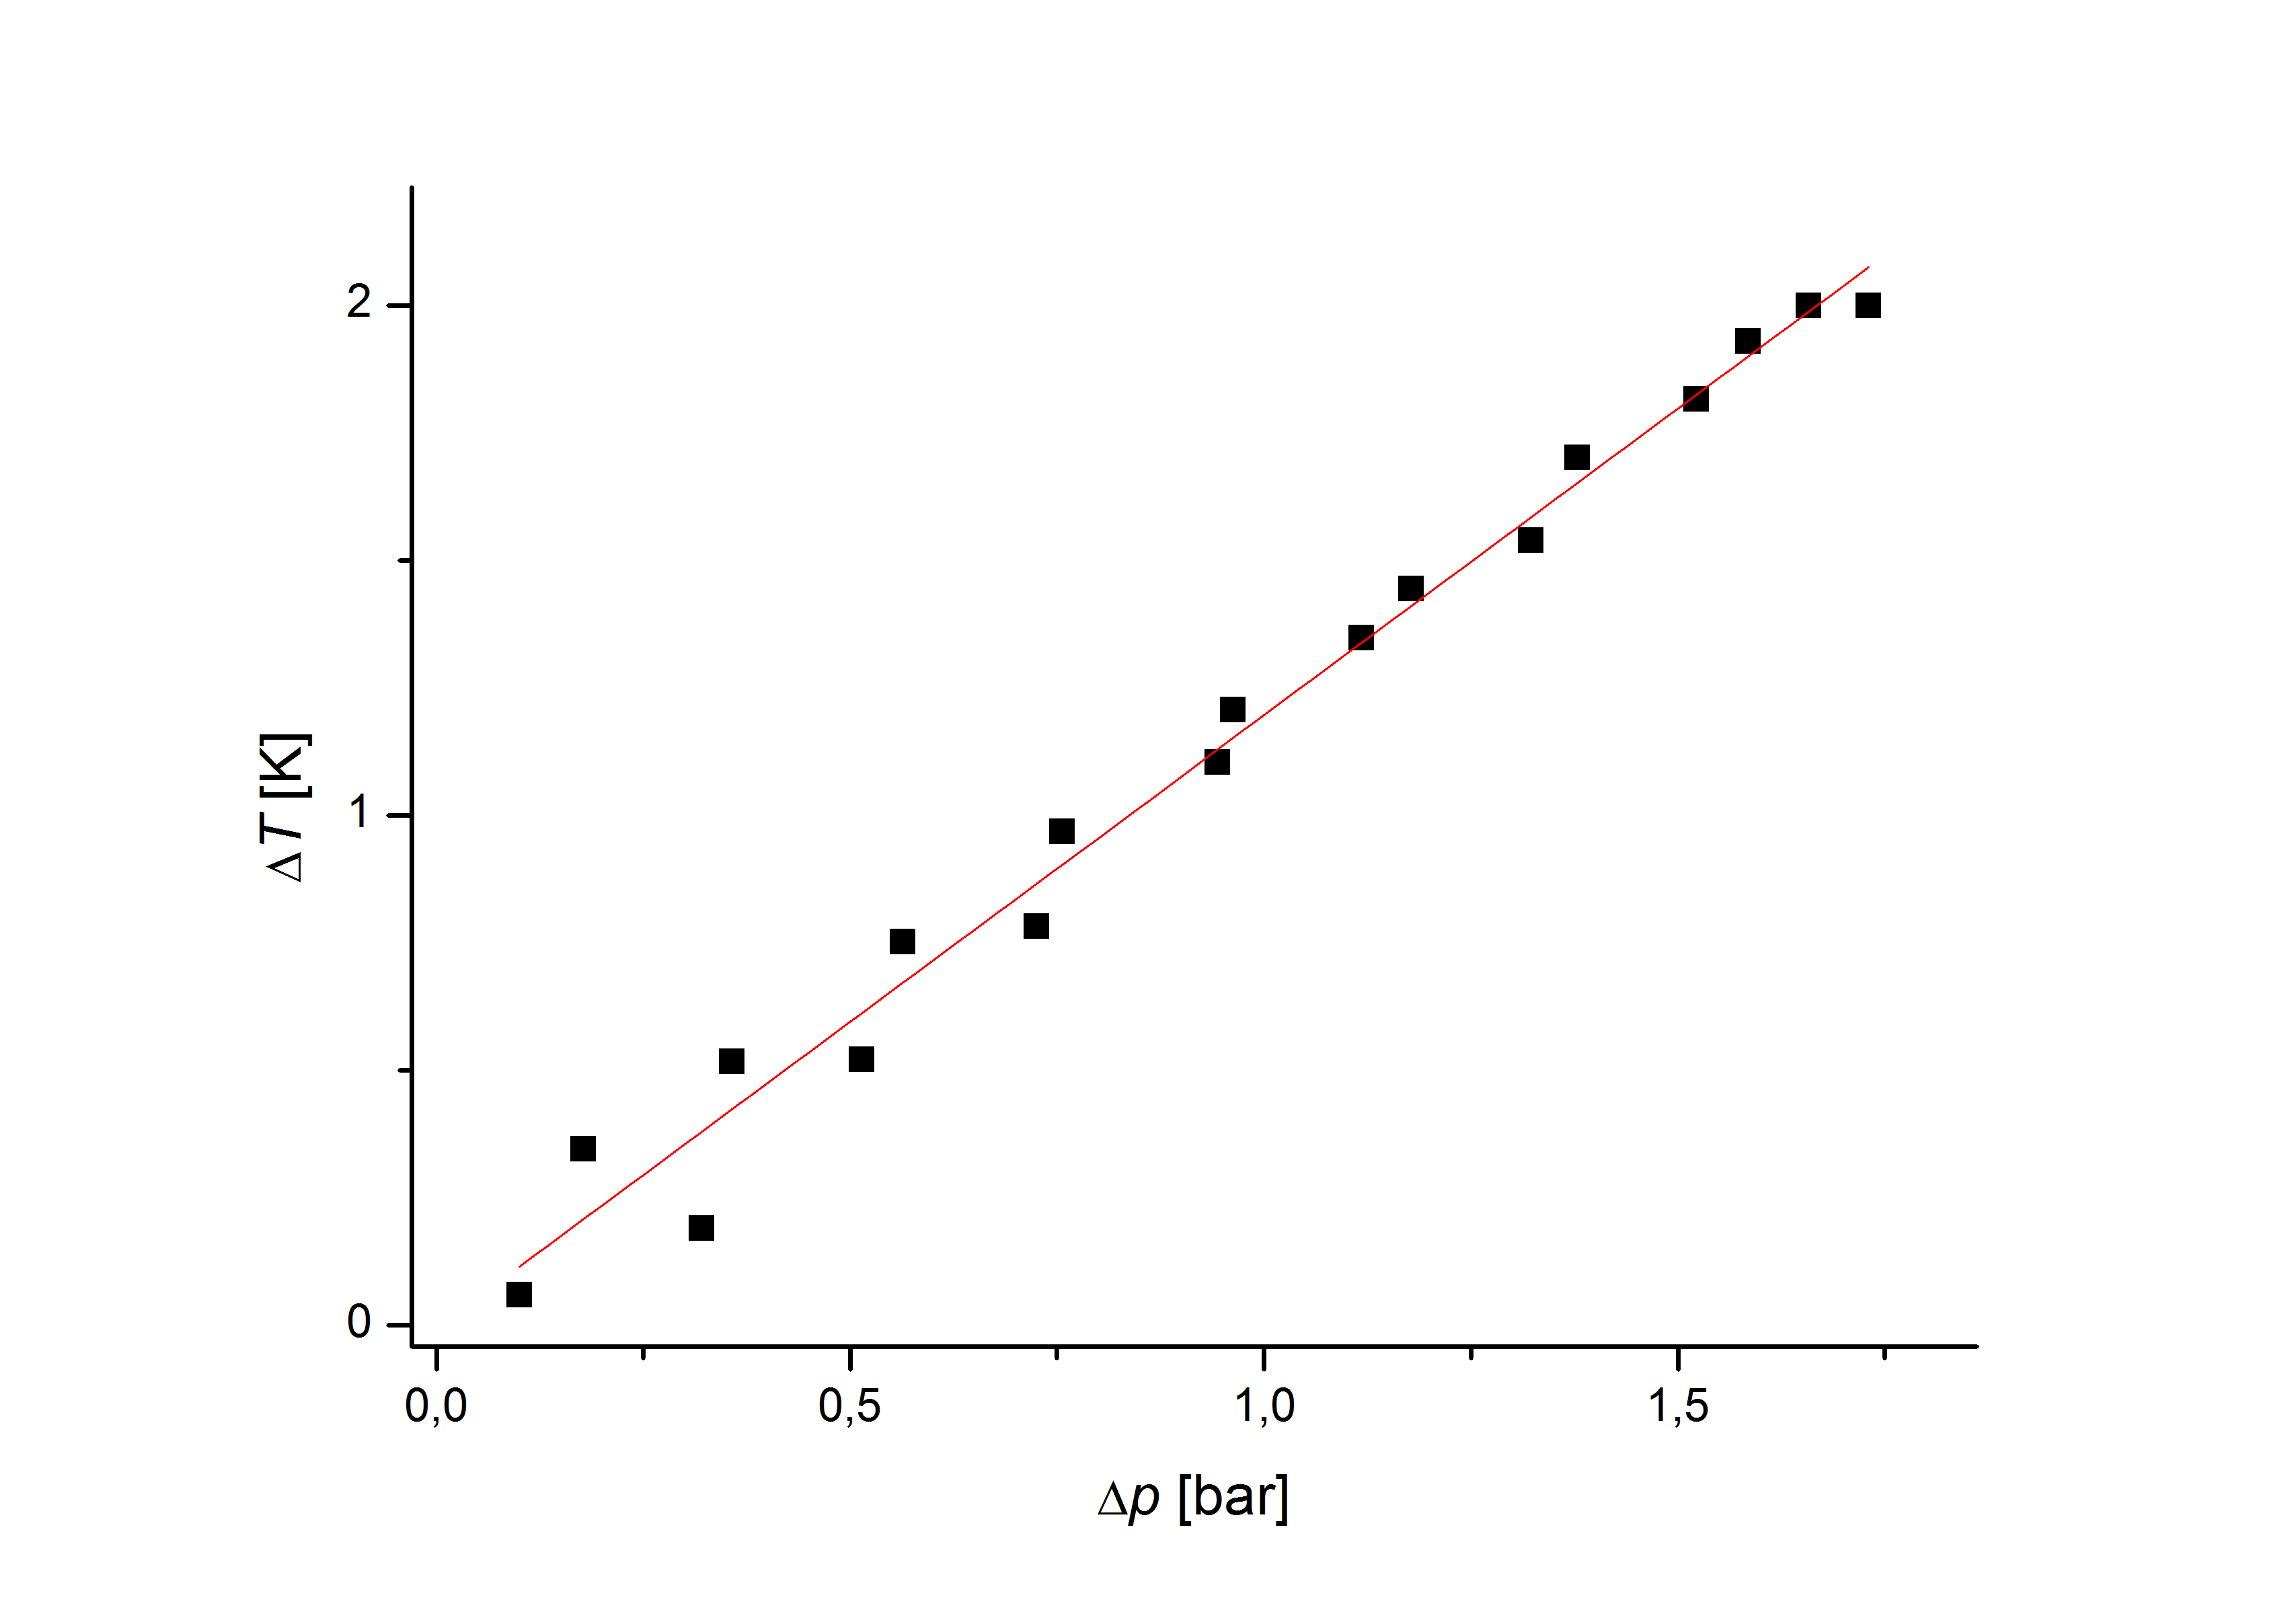
\includegraphics[width=13.5cm]{CO2bei0.png}
\caption{$CO_2$ bei 0,1~°C.}
\end{figure}
\end{center}
\begin{center}
\begin{figure}[h]
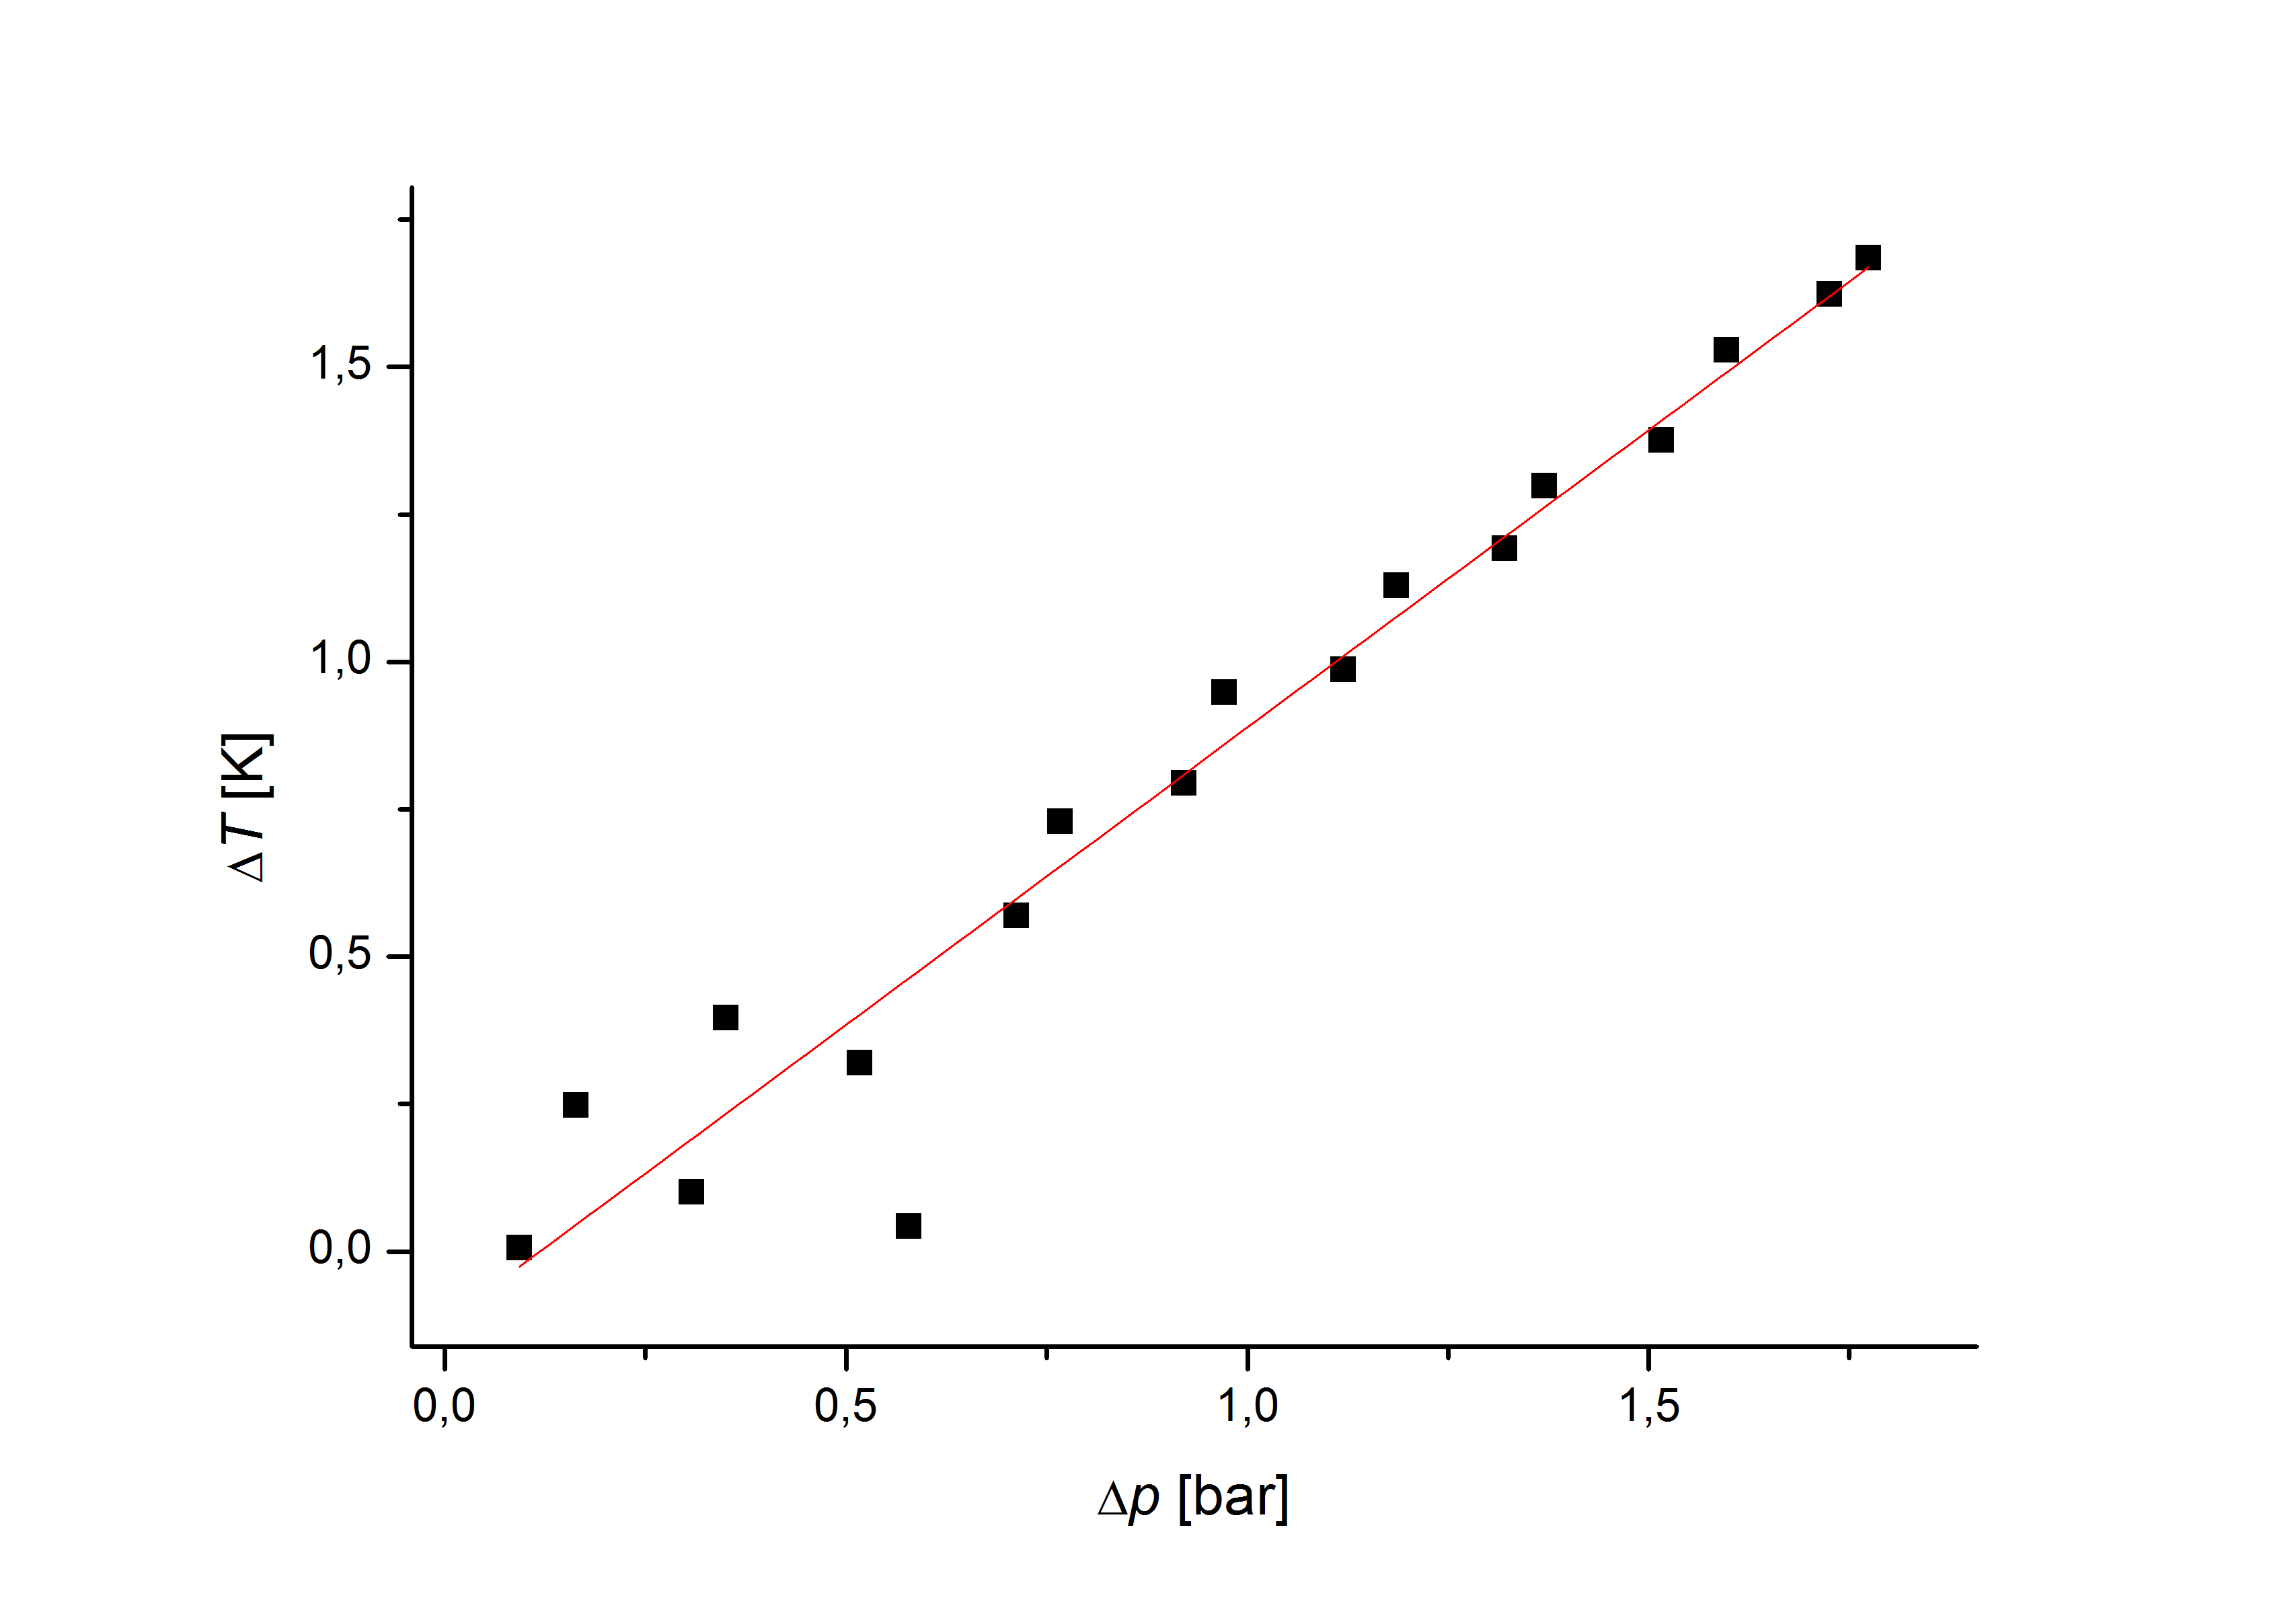
\includegraphics[width=13.5cm]{CO2bei20.png}
\caption{$CO_2$ bei 22,8~°C.}
\end{figure}
\end{center}
\begin{center}
\begin{figure}[h]
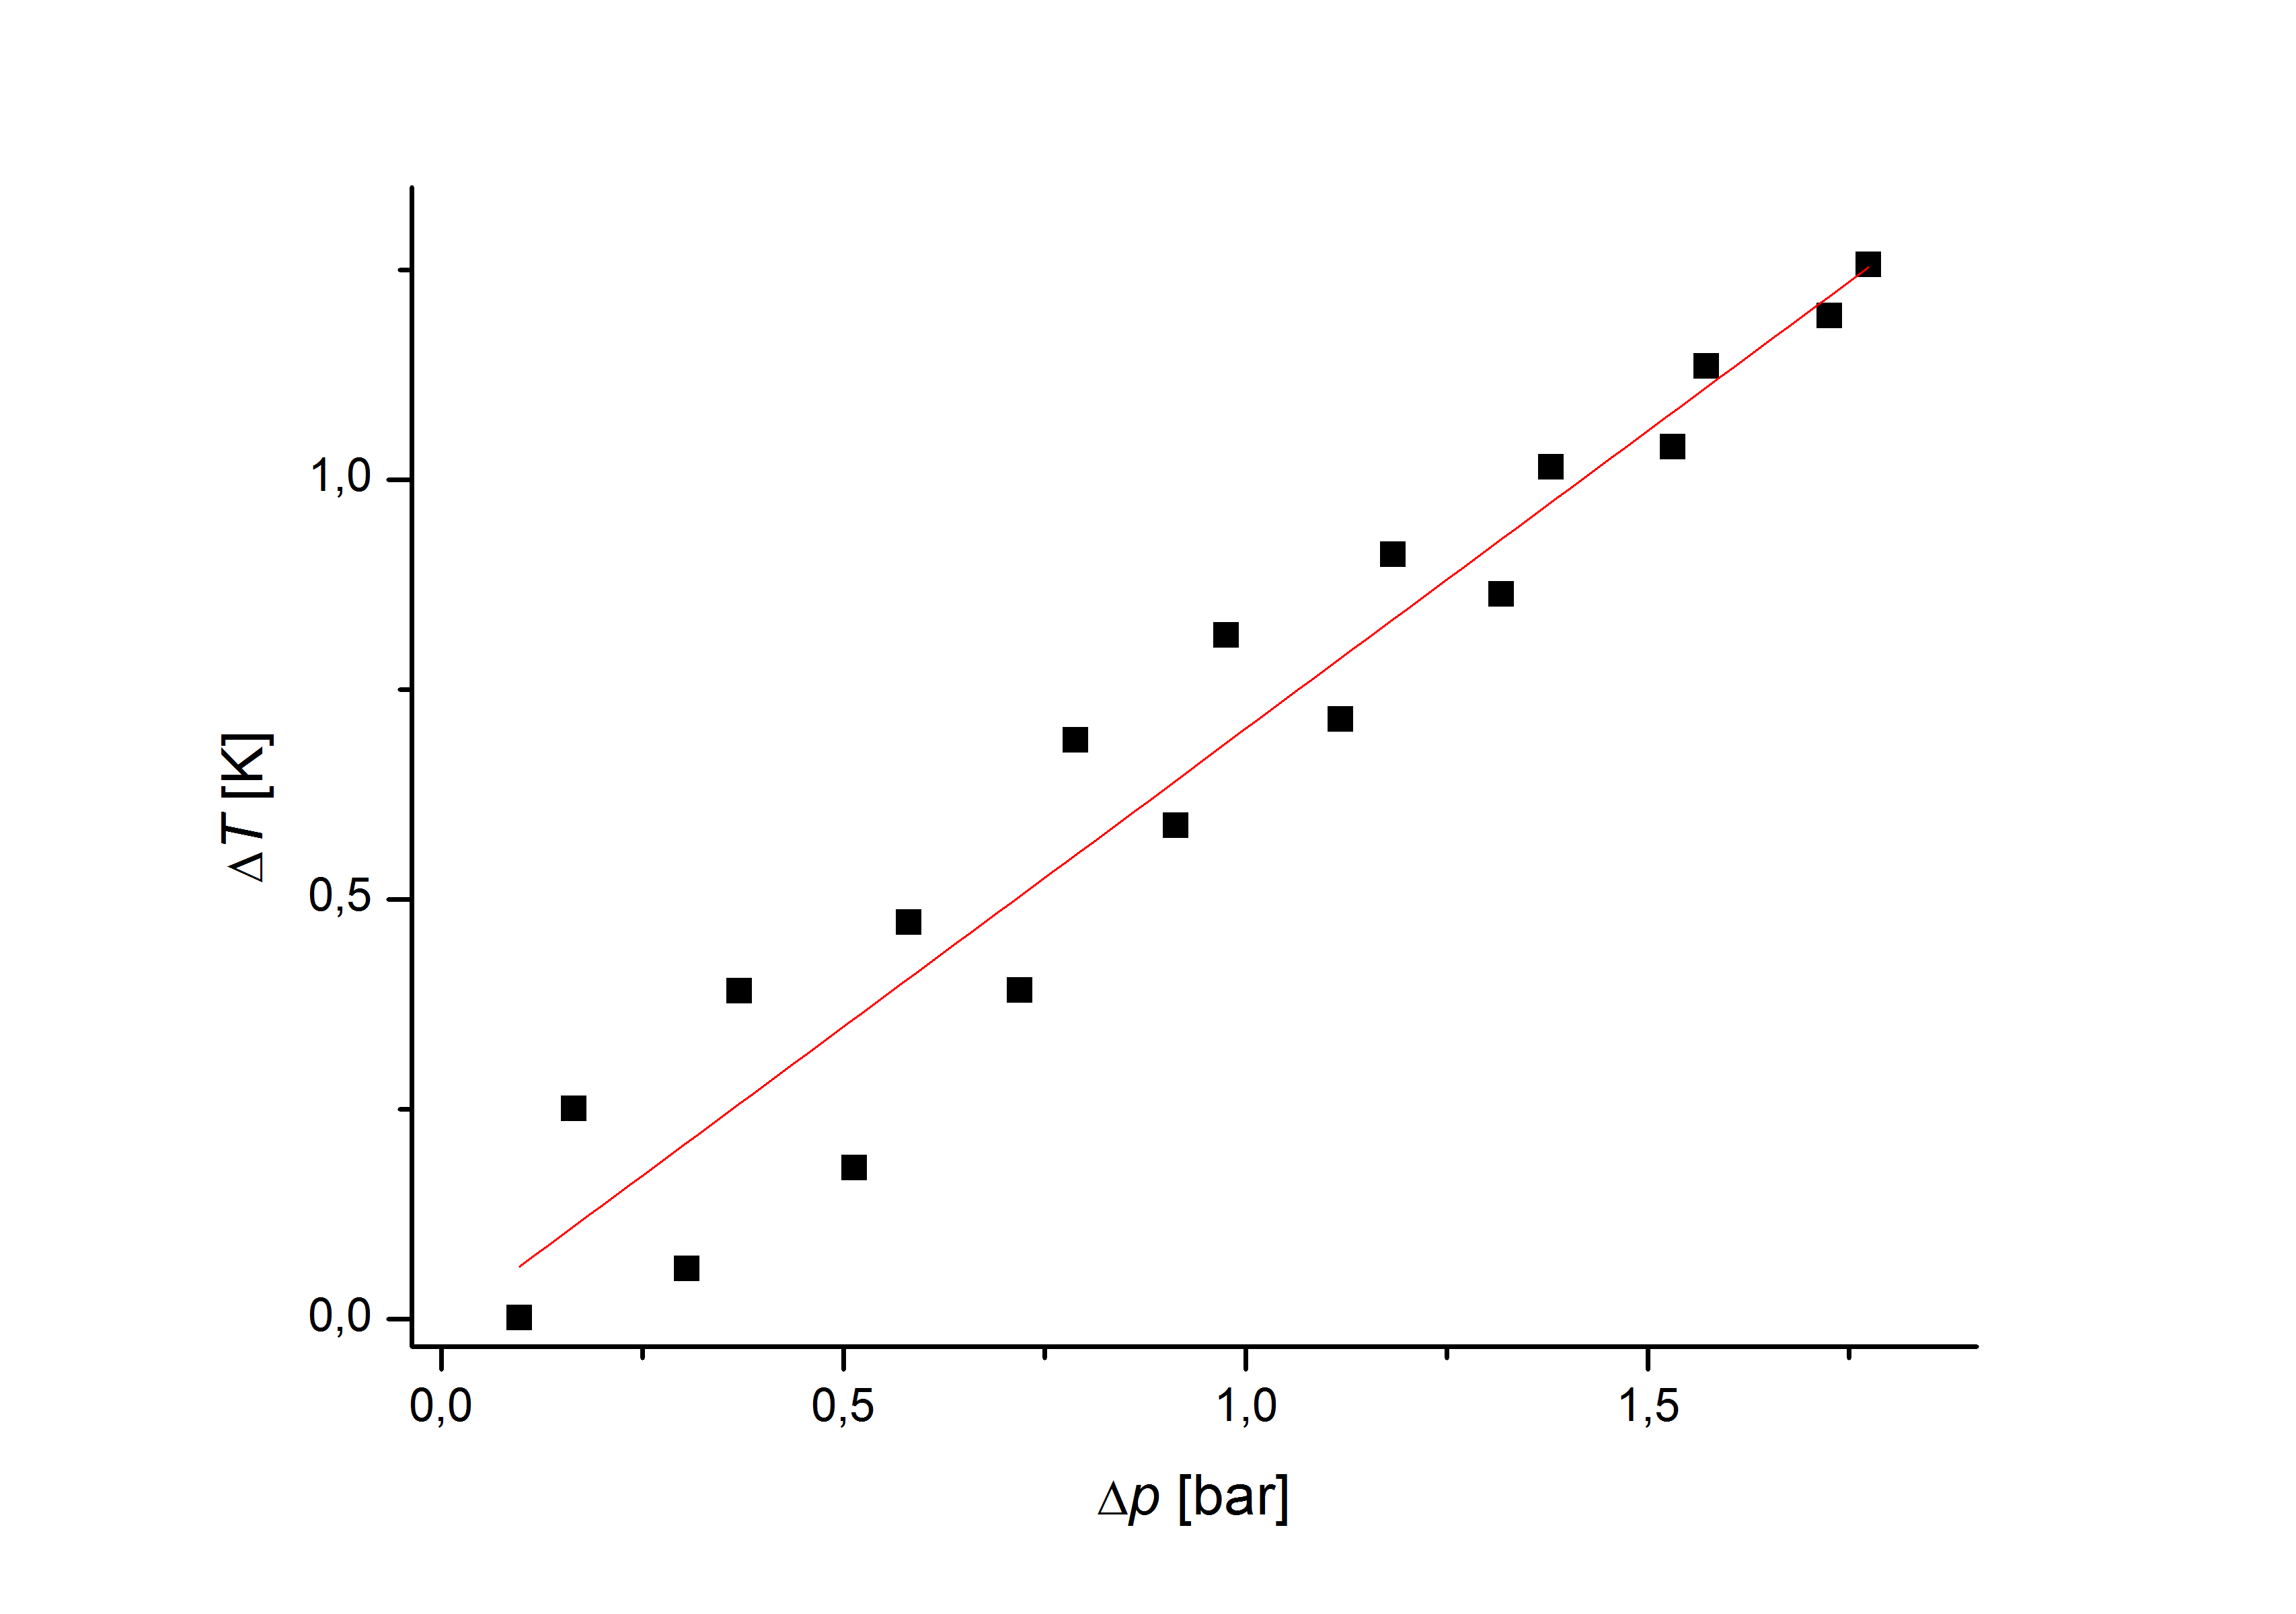
\includegraphics[width=13.5cm]{CO2bei50,8.png}
\caption{$CO_2$ bei 50,8~°C.}
\end{figure}
\end{center}
\newpage




\chapter{Literaturverzeichnis}
1\quad Eckhold, Götz: \emph{Praktikum I zur Physikalischen Chemie}, Institut für Physikalische Chemie, Uni Göttingen, \textbf{2014}.

\vspace{0,5 cm}

2 \quad Eckhold, Götz: \emph{Statistische Thermodynamik}, Institut für Physikalische Chemie, Uni Göttingen, \textbf{2012}.

\vspace{0,5cm}

3 \quad Eckhold, Götz: \emph{Chemisches Gleichgewicht}, Institut für Physikalische Chemie, Uni Göttingen, \textbf{2015}.\\

\vspace{0,5cm}

4 \quad Atkins, P.W.: \emph{Physikalische Chemie}, Wiley-VCH, Weinheim, \textbf{2006}.\\

\vspace{0,5cm}

5 \quad Zemansky: \emph{Heat and Thermodynamics},Mc Graw-Hill, New York, \textbf{1990}.\\

\end{document}
